% ===============================================================================
% \section{Conventions}\label{sec:experiment_conventions}
\section{Motivation}
One of the goals of \wingj is to achieve high level of automation, thus making it easy to use and allowing to spend less time on repetitive and laborious processes. To achieve this, \wingj defines a few conventions such as files naming convention and files organization. Respecting these conventions is also important for running smoothly the \wingj \matlab toolbox introduced in \sectionref{chap:matlab}.

% Finally, a \textit{batch mode} should be released to push the automation even further up to enabling the automatic quantification of one experiment after another.

% ===============================================================================
\section{Experiment name}\label{sec:experiment_name}
An \textit{experiment} refers to the quantification of a single organ system or body system, for instance one \droso wing or embryo. Each experiment must have its own folder from where the input data will be imported and the output data exported. We give below a few examples to illustrate the formatting of the experiment name, which is used to name the experiment folder.

\begin{itemize}
 \item \textbf{20121025\_ch0Name\_114H\_M\_1}. The name of this experiment contains information about the date of the experiment (e.g. the date when the system has been imaged, the format must be yyyymmdd), the number of image stacks or \textit{image channels} and their name (here a single stack called ``ch0Name'' is available), the age of the system (here 114 hours after egg laying) and the index or identifier of the experiment (here M\_1). The age string must end with the character 'H'. Additional examples of age tokens are ``100H'', ``90-91H'', ``114,5-115,5H'', etc. Miscellaneous tokens can be added between the age token and the index of the experiment to provide more information (for example information about the temperature at which the biological system has been imaged).
 \item \textbf{20121025\_ch0Name\_ch1Name\_ch2Name\_ch3Name\_114H\_1}. Same as before but here the name of the experiment reports that there are four image channels (up to four image channels/stacks can be open in \wingj at the same time).
 \item \textbf{20121025\_ch0Name\_ch1Name\_ch2Name\_ch3Name\_114H\_2}. Same as before but here the index reports that it's the second experiment of a batch of experiments.
 \item \textbf{20121025\_mutantName-\_ch0Name\_...\_ch3Name\_114H\-\_1}. The above experiments are supposed to be wild type experiments. If the system imaged is a mutant experiment (e.g. \textit{pent} deficient \droso wing), the name of the mutation followed by a minus sign '-' can be inserted between the date of the experiment and the name of the first image channel. The minus sign is important as it allows \wingj to differentiate the names of the mutations from the names of the channels.
 \item \textbf{20121025\_mutant1Name-\_mutant2Name-\_ch0\-Name\_...\_ch3\-Name\_114H\_1}. Same as before but here there are two mutations. The number of mutations that can be inserted in the name of the experiment is unlimited.
\end{itemize}

\textbf{Tip}: Tokens are separated using underscores '\_'. In general, file and folder names should not include white space ' '. Instead they can be replaced with '\_'.

% ===============================================================================
\section{Experiment directory}\label{sec:experiment_directory}
As mentioned above, the name of an experiment is used to name the \textit{experiment folder}. An experiment folder must contain at least two sub-folders to be identified as such by \wingj in order to automate processes introduced later in this document.

\begin{itemize}
 \item \textbf{images}. Contains the stacks of images, for instance in TIFF format. Most of the microscope softwares allow to export directly or indirectly data in TIFF format (each image of a stack is saved as an individual TIFF file). Additional image stack formats should be supported in the future.
 \item \textbf{WingJ}. This is the output directory where structure and expression datasets should be saved. \wingjMatlab will access this folder later for generating statistics and plots (\sectionref{chap:matlab}), among other tools of \wingj.
\end{itemize}

% ===============================================================================
\section{Experiments root directory}\label{sec:root_directory}
The \textit{experiments root directory} is a folder including many \textit{experiment folders} (\sectionref{sec:experiment_directory}). The name of this directory is the same as the name of the individual experiment folders it includes but without any experiment index or identifier at the end. See \figureref{fig:wingj_benchmark} for an example.

% \begin{itemize}
%  \item \textbf{20121025\_pmadAB\_brkAB\_wg-ptcAB\_114H}
%     \begin{itemize}
%     \item 20121025\_pmadAB\_brkAB\_wg-ptcAB\_114H\_1
% 	\begin{itemize}
% 	\item images
% 	\item WingJ
% 	\end{itemize}
%     \item 20121025\_pmadAB\_brkAB\_wg-ptcAB\_114H\_2
% 	\begin{itemize}
% 	\item images
% 	\item WingJ
% 	\end{itemize}
%     \item 20121025\_pmadAB\_brkAB\_wg-ptcAB\_114H\_3
% 	\begin{itemize}
% 	\item images
% 	\item WingJ
% 	\end{itemize}
%     \end{itemize}
% \end{itemize}

% ===============================================================================
\section{Experiments repository}\label{sec:experiment_repository}
The \textit{experiments repository} is a folder that contains many \textit{experiments root directory} (\sectionref{sec:root_directory}). Its name can be chosen freely.\\

To illustrate the above organization of folders, we show in \figureref{fig:wingj_benchmark} the typical content of an \textit{experiments repository} which contains \textit{experiments root directories}, which themselves contain many individual \textit{experiments} each. Remember that one experiment correspond to a single instance of a system, for instance one wing or one embryo.

\begin{figure}[!h]
\centering
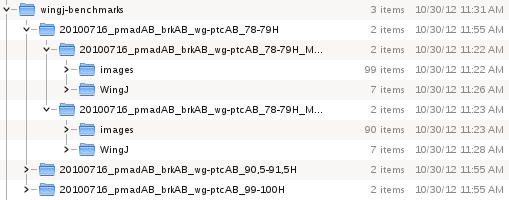
\includegraphics[scale=0.75]{images/wingj_benchmark.jpg}
\caption{\textbf{Illustration of the organization of experiment folders for automating processes in \wingj.} Here the experiments repository is named ``wingj-benchmarks'' and matches the content of the \wingjBenchmarkImages. The repository contains several experiments root directories that each represents a type or class of experiments. Here there are three classes of experiments corresponding to different time points at which the wings have been imaged (about 78h-, 91h-, and 100h-old wings). Finally, each experiment folder contains the two sub-folders \textit{images} (contains the input images in TIFF format) and \textit{WingJ} (output folder for exporting datasets from \wingj).}
\label{fig:wingj_benchmark}
\end{figure}

% ===============================================================================
\section{Channel name} \label{convention_experiment_channel_names}
Up to four image stacks can be open at the same time in \wingj. Each image stack typically corresponds to a single \textit{color channel} (or \textit{image channel}. Depending on the color space used by the microscope software to export the images, each image exported will contain more or less channels. For instance, RGB (red, gree, and blue) images are made out of three channels when CMYK (cyan, magenta, yellow, and black) color space produces images including four channels. Considering RGB encoding, each image taken by the microscope is made of three individual images, each encoding the information from a different color.\\

Image channels are given names in \wingj to identify them without ambiguity. The channel name is also used to export the expression datasets obtained from the quantification of a selected image channel. We give below a few examples of channel names:\\

``dadGFP'', ``brkGFP'', ``wg-ptcAB'', ``wg-ptcGAL4'', ``wg-ptcLACZ'', etc.\\

Use lowercase letters for the name of the gene/protein visible in the image channel. Use the minus sign '-' to separate multiple gene/protein names (e.g. ``wg-ptc'' stands for \textit{wingless} and \textit{patch} proteins). Uppercase letters are then used to denote the fluorescence techniques used (GFP=Green Fluorescent Protein, AB=Antibody, etc.).\\

\textbf{Tip}: The respect of the above file organization is particularly important for the \textit{aggregation of structure and expression models} introduced in \sectionref{sec:community_expression_maps}. More information are available in the \textit{Support} section of the project website (\wingjShortUrl).\\

\textbf{Tip}: We invite you to download the \wingjBenchmarkImages to have a concrete example of a directory structure following the \wingj naming conventions.

% \subsection{Confocal image filenames} \label{sec:convention_image_filenames}
% The format used for image filenames matches the format used by most of the confocal microscopes. In our experiments, we use a confocal microscope \textit{Leica SP5} and exported the images in TIFF format with the software \textit{Leica Application Suite}. This allows \wingj to be immediately used without having to rename the exported images. Confocal image filenames are formatted as below:\\
% 
% \textit{NAME}\_ZSLICE\_CHANNEL.tif\\
% E.g ``Series003\_z05\_ch01.tif''\\

% Note that all the elements contained in an image filename must be separated by underscores (\_). \textit{NAME} represents any name string. The two important elements are:
% 
% \begin{mylist}
%  \item \textbf{ZSLICE}\\Provides information about the current z-slice. \textit{ZSLICE} must be replaced in the above format by ``z00'', ``z01'', ..., ``z56'', ``z57'', etc.\\
% 
%  \item \textbf{CHANNEL}\\Provides information about the current channel. \textit{CHANNEL} must be replaced in the above format by ``ch00'', ``ch01'' and ch02``. If a fourth channel is present, ''ch03`` is used. The first channel must always be ch00 (and not ch01). Furthermore, ch00 must correspond to the red channel (R), ch01 to the green channel (G) and ch02 to the blue channel (B). If four channels are used, ch00 to ch03 must correspond to the four colors cyan (C), magenta (M), yellow (Y) and key black (K).
% \end{mylist}


% . In \textit{Normal} mode, any experiment names will do the job. In general, it is recommended to not use white space ' ' in filenames (replace by '\_'). In \textit{Batch} mode, it is important to respect the format defined in Section XXX. It is also recommended to use that format for experiments in \textit{Normal} mode. An example of experiment name following the format given in Section XXX is:\\